\chapter{Quantum Optimal Control}\label{chap:3_Quantum_Optimal_control}



Natural and foremost questions for engineering quantum technological devices are ‘what can one do with them?’, in particular ‘which states can be prepared?’ or ‘which quantum gates can be implemented?’ Answering these questions connects engineering with the core of mathematical control theory.

\reminder{something something control objectives: state preparation, protection against decoherence, gate synthesis/optimisation, entanglement generation, enhanced measurements}

\reminder{what do you want to achieve $\rightarrow$ what is the quantitative formula for achieving this?}

Good citations to have in here: \cite{schirmer_complete_2001, koch_quantum_2022,glaser_training_2015}


\section{The structure of optimal control problems}\label{sec:3.1_structure_quantum_control}

The idea of an optimal control problem is simple: envision a target you want to achieve, cast it into some form of quantitative or abstract mathematical formula and then use said formula to derive the `best' path to get to said objective. The aim of the first part of this section is thus to broadly cover the mathematical structure of optimal control problems and then, in the second, to delve more into practical questions of controllability and the process of optimisation.

\subsection{Mathematical structure}\label{sec:3.1.1_mathematical_structure}

In general, an optimal control problem is composed of a set of state functions $X: \R \rightarrow \R^n$, and a set of time-dependent control functions $U:\R \rightarrow \R^m$ and the optimal control problem consists of finding $x \in X$ and $u \in U$ that minimise some functional $C: X \cross U \rightarrow \R$ such that the constraint:
\begin{equation}\label{eq:control_ODE}
    \dot{x} = f(x, u),
\end{equation}
is satisfied almost everywhere. This is a very abstract description and just about any control problem can be expressed as a special case of this formulation \cite{dalessandro_introduction_2021}. To gain more intuition, we can imagine a more concrete example where, \@~e.g. $U$ and $X$ are sets of continuous functions on the interval $[0, \tau]$ satisfying $x(0) = x_0$. In this scenario, $\tau$ could be a time interval during which we want to drive the system from an initial state $x_0$ to a final state $x_f$ using the control function $u(t)$, $t \in [0, \tau]$. The choice of functional $C$ would have to capture the desired outcome of the protocol: that the state of the system after the driving $x(\tau)$ be equal to the target $x_f$. This can be done by choosing a distance metric that depends on only on the drive $u$ and is minimised when $x(\tau) = x_f$, \@~e.g.
\begin{equation}\label{eq:example_cost_func}
    C(u) = \norm{x(\tau)  - x_f}^2.
\end{equation}
The functional $C$ is often referred to in literature as the \emph{cost} or \emph{loss} function \cite{wald_statistical_1950} as it encodes the quality of the final protocol with respect to the desired outcome of the protocol. In that sense, we can imagine adding constraints to the problem that may increase the `cost' of the protocol output if they are not satisfied to some degree. For example, Eq.~\eqref{eq:example_cost_func} can be modified to include additional terms:
\begin{equation}\label{eq:example_cost_func2}
    C(u) = \gamma \norm{x(\tau)  - x_f}^2 + \int_0^{\tau} \norm{u(t)}^2 dt,
\end{equation}
where $\gamma$ is a penalty term on the final state that scales its importance relative to the additional second term, which is analogous to the cost in the energy required to achieve the final state. This updated cost function can be read as introducing a competition between the quality of the final state and the amount of energy expended to get it there, mediated by the value of $\gamma$. 

\begin{figure}[t]
\centering
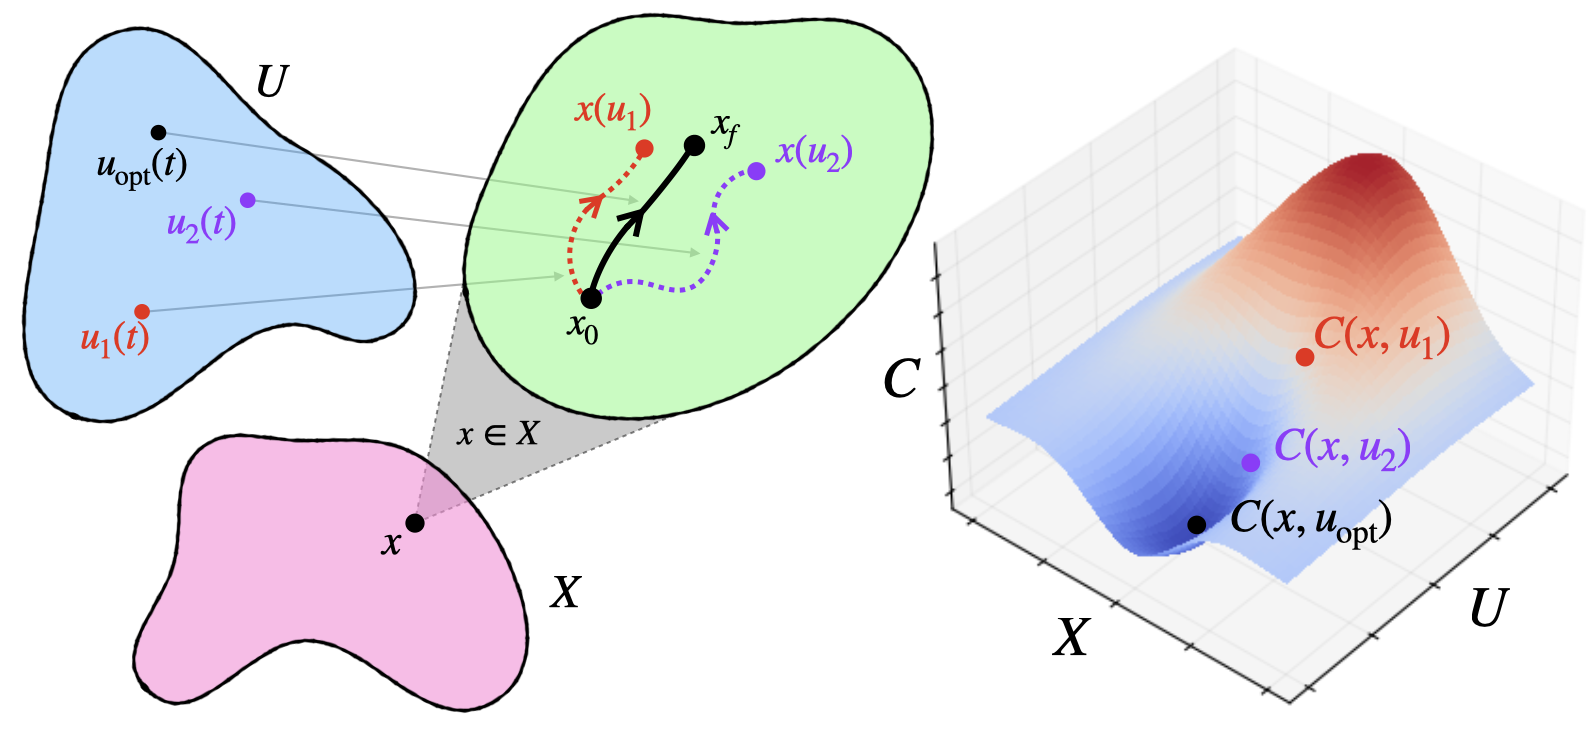
\includegraphics[width=0.9\linewidth]{images/optimal_control_illustration.png} \caption[Illustration of optimal control problem structure]{Illustration of the Mayer type optimal control problem: when an initial value of the system state $x_0$ is fixed, the choice of control function $u \in U$ and the requirement of satisfying Eq.~\eqref{eq:control_ODE} determine $x$ uniquely. The task is then to find $u_{\rm opt}$ such that the functional $C(x, u_{\rm opt})$ is minimised.}\label{fig:optimal_control}
\end{figure}

There are several different types of problem structures in optimal control centering on different constraints and targets (see \Cref{box:mayerbox}). In this thesis, we will primarily focus on what are often called \emph{Mayer-type} problems\cite{dalessandro_introduction_2021}, where the initial state is specified $x(0) = x_0$ and the cost function is of the form
\begin{equation}\label{eq:mayer_costfunc}
    C(u) = \phi(x(\tau), \tau),
\end{equation}
where $\phi$ is a smooth function and $\tau$ the total time of the protocol. These two constraints and the requirement given by Eq.~\eqref{eq:control_ODE} define the state function $x$ uniquely and the problem is then to determine a control function $u$ on the appropriate set $[0, \tau]$ which minimises Eq.~\eqref{eq:mayer_costfunc}. In Mayer-type problems, a specific target state can be defined in the cost function as a constraint, which is the case in Eq.~\eqref{eq:example_cost_func} and this is illustrated in Fig.~\ref{fig:optimal_control}. However, this need not be the case as target states can be made implicit by having the cost function instead target some property of the state instead, like Euclidean distance from the initial state. 

\begin{mycolorbox}[box:mayerbox]{{Mayer, Lagrange and Bolza}}
    There are primarily three types of optimal control problems: \textbf{Mayer}, \textbf{Lagrange} and \textbf{Bolza}. In the main text we cover the Mayer-type problem in detail, but it is useful to understand what differentiates it from the others.
    \begin{enumerate}
        \item Mayer-type problems are ones that are primarily concerned with the final state of the system and not its trajectory, with cost functions of the form given in Eq.~\eqref{eq:mayer_costfunc}.
        \item Lagrange-type problems are ones where the focus is on the behaviour of the system throughout the trajectory and they encompass cost functions of the type
        \begin{equation}
            C(u) = \int_0^{\tau} L(x, u, t) dt
        \end{equation}
        where $L$ is a smooth function. 
        \item Bolza problems are a combination of the two, where both the system's behaviour during the trajectory and its final state matter:
        \begin{equation}
            C(u) = \phi(x(\tau), \tau) + \int_0^{\tau} L(x, u, t) dt,
        \end{equation}
        where $\phi$ is a smooth function as given in Eq.~\eqref{eq:mayer_costfunc}. Bolza problems are thus more general and flexible, with the cost function in Eq.~\eqref{eq:example_cost_func2} serving as a great example.
    \end{enumerate}
\end{mycolorbox}

Apart from identifying the basic anatomy of control problems in terms of $X$, $U$ and $C$, there is a myriad of additional information about their mathematical structure that can help to analyse and thus solve them. For example, it might be useful to identify if, for a particular optimal control problem, the system in question is \emph{controllable}\cite{dirr_lie_2008, fleming_optimal_1975} \@i.e.~can any initial state be transformed into any desired target state. Equally, it might be useful to study what are called \emph{reachable sets}\cite{vom_ende_reachability_2020, fleming_optimal_1975}, which are sets containing all the states that an initial state can be driven to by the set of control functions $U$. In the case of Mayer-type problems, for example, it might be sensible to define a reachable set parameterised by the final evolution time $\tau$ such that it contains all possible states that can be obtained by the system during a driving time $\tau$. Finally, I would be remiss not to mention the concept of \emph{necessary conditions for optimality}\cite{mangasarian_sufficient_1966}, which focus on determining what formal conditions need to be satisfied for a specific control $u \in U$ to be optimal. Generally, this involves perturbing an assumed optimal control $u$ by some small parameter $\epsilon$ giving $u^{\epsilon}$ and then imposing the constraint that
\begin{equation}\label{eq:optimality_condition}
    C(u^{\epsilon}) - C(u) \geq 0,
\end{equation}
which is then considered the necessary condition for optimality. The most basic of these optimality conditions is the Pontryagin maximum principle or \acrref{PMP} \cite{boltyanski_nonclassical_1999} (see \Cref{box:pontryagin}), which states that for an optimal control problem, the optimal control and state trajectories should maximize a specific function which combines the system dynamics, the control inputs, and the Lagrange multipliers which encode the constraints of the control problem.

\subsection{Analytic optimisation}

While the first part of optimal control is the construction of the problem, the second part is the search for a solution. The methods used to do this can generally be classified either as analytic or numerical approaches. While both are widely used in optimal control theory, this thesis will largely only focus on the latter, so I will be brief in introducing the former. 

Analytic optimal control techniques are those that leverage mathematical rigor and formalism to derive solutions or insights, as opposed to relying primarily on numerical simulations, heuristics, or experimentation. They provide a theoretical foundation for understanding the properties and solutions of optimal control problems and are closely related to the discussion in Sec.~\ref{sec:3.1.1_mathematical_structure}. They can allow for a complete geometric understanding of the control problem leading to, for example, knowledge of the structure of a solution or even some proof about a global optimum. For a given set of constraints they might even be used to derive time limits of state transformations, \@i.e.~ the concept of reachability that I discuss in a little more detail in \Cref{box:reachability} in the case of quantum systems. An example of analytic methods is the aforementioned \acrref{PMP}, which provides a means to solve optimal control problems by reducing them to a set of differential equations.

\begin{mycolorbox}[box:pontryagin]{Pontryagin maximum principle}
    For Mayer-type problems of Eq.~\eqref{eq:mayer_costfunc}, the \acrref{PMP} is defined as:
    \begin{theo}{{\acrref{PMP} for Mayer problems}}
        FFor fixed final time $\tau$ and free final state assume $u$ is the optimal control and $x$ the corresponding trajectory solution of Eq.~\eqref{eq:control_ODE}. Then, there exists a nonzero vector $\lambda$ solution of the adjoint equations
      \begin{equation}
          \dotlambda^T = - \lambda^T f(x(t), u(t))
      \end{equation}
      with terminal condition
      \begin{equation}
          \lambda^T(\tau) = -\phi(x(\tau))
      \end{equation}
      such that, for almost every $t \in (0, \tau]$, we have
      \begin{equation}\label{eq:pmp_maximisation}
          \lambda^T(t) f(x(t), u(t)) \geq \lambda^T(t) f(x(t), v)
      \end{equation}
      for every $v$ in the set of the admissible values for the control $U$. Furthermore, for every $t \in [0, \tau]$
      \begin{equation}\label{eq:pmp_constant}
          \lambda^T(t) f(x(t), u(t)) = c,
      \end{equation}
      for a constant $c$
    \end{theo}
    Using this, one can then define the \emph{optimal control Hamiltonian}:
    \begin{equation}
        h(\lambda, x, u) := \lambda^T(t) f(x, u).
    \end{equation}
    Now we can recast Eqs.~\eqref{eq:pmp_maximisation} and \eqref{eq:pmp_constant}:
    \begin{equation}
        \begin{aligned}
            h(\lambda(t), x(t), u(t)) &= c \\
            h(\lambda, x, u) &\geq h(\lambda, x, v),
        \end{aligned}
    \end{equation}
    where the second equation is essentially maximising $h$ over $u \in U$ for each $\lambda$ and $x$. The solution will thus be of the form $u := u(x, \lambda)$ and it can be solved with the system of equations
    \begin{equation}
        \begin{aligned}
            \dot{x} &= f(x, u(x, \lambda)), \\
            \dotlambda^T &= -\lambda^T f(x, u(x, \lambda))
        \end{aligned}
    \end{equation}
    with the boundary conditions $x(0) = x_0$ and $\lambda^T(\tau) = -\phi(x(\tau))$. The kicker is that every control which is obtained with this procedure satisfies the necessary conditions of optimality and it is a candidate to be the optimal control.
    
\end{mycolorbox}

The trouble with analytic approaches, despite the commonplace rigorous guarantees of optimality and the scope of information they provide about the system, trajectory and structure of the control problems and their solutions, is that they are very difficult to scale up and quite inflexible to complex problem constraints. As such, analytic approaches are generally reserved for special cases, when problems have low dimensionality and simple structures where the cost function is generally linear in the arguments. Many real-world control systems require more complexity and flexibility than can be afforded by analytic methods.

\subsection{Numerical optimisation} 

To overcome the drawbacks of analytic approaches, many optimal control problems are instead solved using numerical optimisation methods. These are generally algorithmic, iterative  techniques which explore the cost function landscape step-by-step in order to converge to a minimum value. Numerical methods generally do not offer the same analysis or guarantees of optimality that analytic methods do. Their iterative nature may lead to a dependence of the outcome on the initial conditions of the algorithm, such as an initial guess for an optimal solution from which the iterations proceed or the bounds on the search space. Despite these drawbacks, however, 

A general numerical optimisation technique consists of an initialisation step, a series of search steps and a termination step. These can be summarised as follows:
\begin{enumerate}
    \item \emph{Initialisation}: set up the necessary constraints of the optimal control problem, such as bounds on the solution space or an initial guess for the optimal solution.
    \item \emph{Search}: Perform some iterative search steps (deterministic or stochastic) with the goal of converging to the minimum of the cost function. What constitutes a single step varies massively between different techniques.
    \item \emph{Termination}: Return a solution after some condition is satisfied. This can be a convergence criterion based on the change in the cost function value between steps or a limit on the number of search steps that the algorithm is allowed to perform.
\end{enumerate}

The simplicity of these three components leaves a lot of room for creativity and over the years many numerical optimisation algorithms and techniques have been developed to deal with different constraints and topologies of different cost function landscapes. It would take an entire book to cover the various categories and subcategories that exist within the field, so I will restrict myself to exploring a few key classifications of the structure of numerical optimisation methods. 

One of the more broad ways to classify numerical optimisation methods is into the categories of \emph{gradient-based} methods and \emph{gradient-free} methods. Gradient-based methods, as the name implies, make use of gradient information (the first derivative of the cost function) to guide the search for an optimal solution. These methods are often efficient and converge rapidly when the cost function is smooth and differentiable. A popular example of a gradient-based method is the gradient descent algorithm, which iteratively adjusts the solution in the direction opposite to the gradient, as this direction is likely the steepest decrease in the cost function value. A typical gradient descent protocol might look like:
\begin{equation}\label{eq:gradient_descent}
    \ubb_{t + 1} = \ubb_t - \mu \grad_{\ubb} C(\ubb),
\end{equation}
where $t$ denotes the current iteration of the algorithm, $\grad_{\ubb} C(\ubb)$ is the derivative of the cost function $C$ with respect to the control parameters $\ubb$ and $\mu$ is generally known as the `learning rate' or `step size' and its job is to control the resolution at which the algorithm traverses the cost landscape. Larger $\mu$ might lead to faster convergence but it might also mean overshooting the cost function minimum, so adjusting its value is often a heuristic that requires some experimentation. Other examples of gradient-based methods include Newton's method and quasi-Newton methods \cite{suli_introduction_2003}, which employ information about the second derivative to guide the search and provide faster convergence as well as a myriad of other approaches including stochastic methods \cite{bottou_tradeoffs_2007}. 

Gradient-free methods, on the other hand, do not require gradient information, making them suitable for optimization problems where the cost function is, \@e.g.~ discontinuous, non-differentiable, or its gradient is difficult or expensive to compute. Examples of gradient-free methods include particle swarm optimization\cite{bonyadi_particle_2017}, the Nelder-Mead method, which I will explore in more detail in Sec.~\ref{sec:3.1.3.1_Nelder_Mead} as well as the Powell method of Sec.~\ref{sec:3.1.3.2_Powell}. These methods often rely on trial and error, random sampling, or mimicking natural phenomena like evolutionary mechanisms\cite{vikhar_evolutionary_2016} to explore the solution space. As in the case of gradient-based approaches, there is a veritable zoo of methods under this umbrella. As the rest of this thesis we will deal almost exclusively with gradient-free methods, I will provide examples of how these techniques look in the next couple of sections.

\begin{mycolorbox}[box:openclosedloop]{{Open-loop vs. closed-loop optimisation}}
    When dealing with real-world control systems, 
\end{mycolorbox}

Apart from the gradient-information, another key way to classify optimisation algorithms is either as \emph{local} or \emph{global}. Local optimization methods are designed to find a local minimum, which is a solution that is better than all other feasible solutions in its vicinity in the landscape of the cost function. They are typically efficient at converging to the local minimum, but they provide no guarantee of finding the global minimum if the cost function is non-convex \@i.e. the local minimum is not automatically also the global minimum. Both Nelder-Mead and Powell are local methods.

Global optimization methods, on the other hand, aim to find a global optimum, which is the best solution among all feasible solutions, not just those in a local neighborhood. These methods typically employ a strategy to explore the entire solution space, either deterministically or stochastically, to avoid getting trapped in a local optimum. As a result of this larger scope, global optimization methods are generally more computationally intensive than local methods. An example of global optimisation that I will explore in more detail in Sec.~\ref{sec:3.1.3.3_dual_annealing} is Dual-Annealing, which combines generalized simulated annealing\cite{tsallis_generalized_1996}, a global search algorithm, with local optimisers in order to find an optimal solution. Global methods are often used when the optimization problem is complex, non-convex, or the global solution is significantly better than any local solution.

There are many

\subsubsection{Nelder-Mead}\label{sec:3.1.3.1_Nelder_Mead}

A frequently used gradient-free optimisers is Nelder-Mead (or downhill-simplex) method \cite{nelder_simplex_1965} developed by J. Nelder and R. Mead in 1965. It is what's known as a \emph{direct search} or \emph{pattern search} approach and it is a gradient-free local method, making it generally quite efficient, but not guaranteed to converge to a global optimum of the cost function. Direct search methods work by varying each optimisable parameter by some small stepsize from the current minimum in each direction and computing the cost function at the updated value. The change that leads to the largest decrease in the cost function value is taken as the new minimum. Once no such variation leads to an improvement, the stepsize is halved and the process is repeated until some convergence criterion is satisfied.

\begin{figure}[t]
\centering
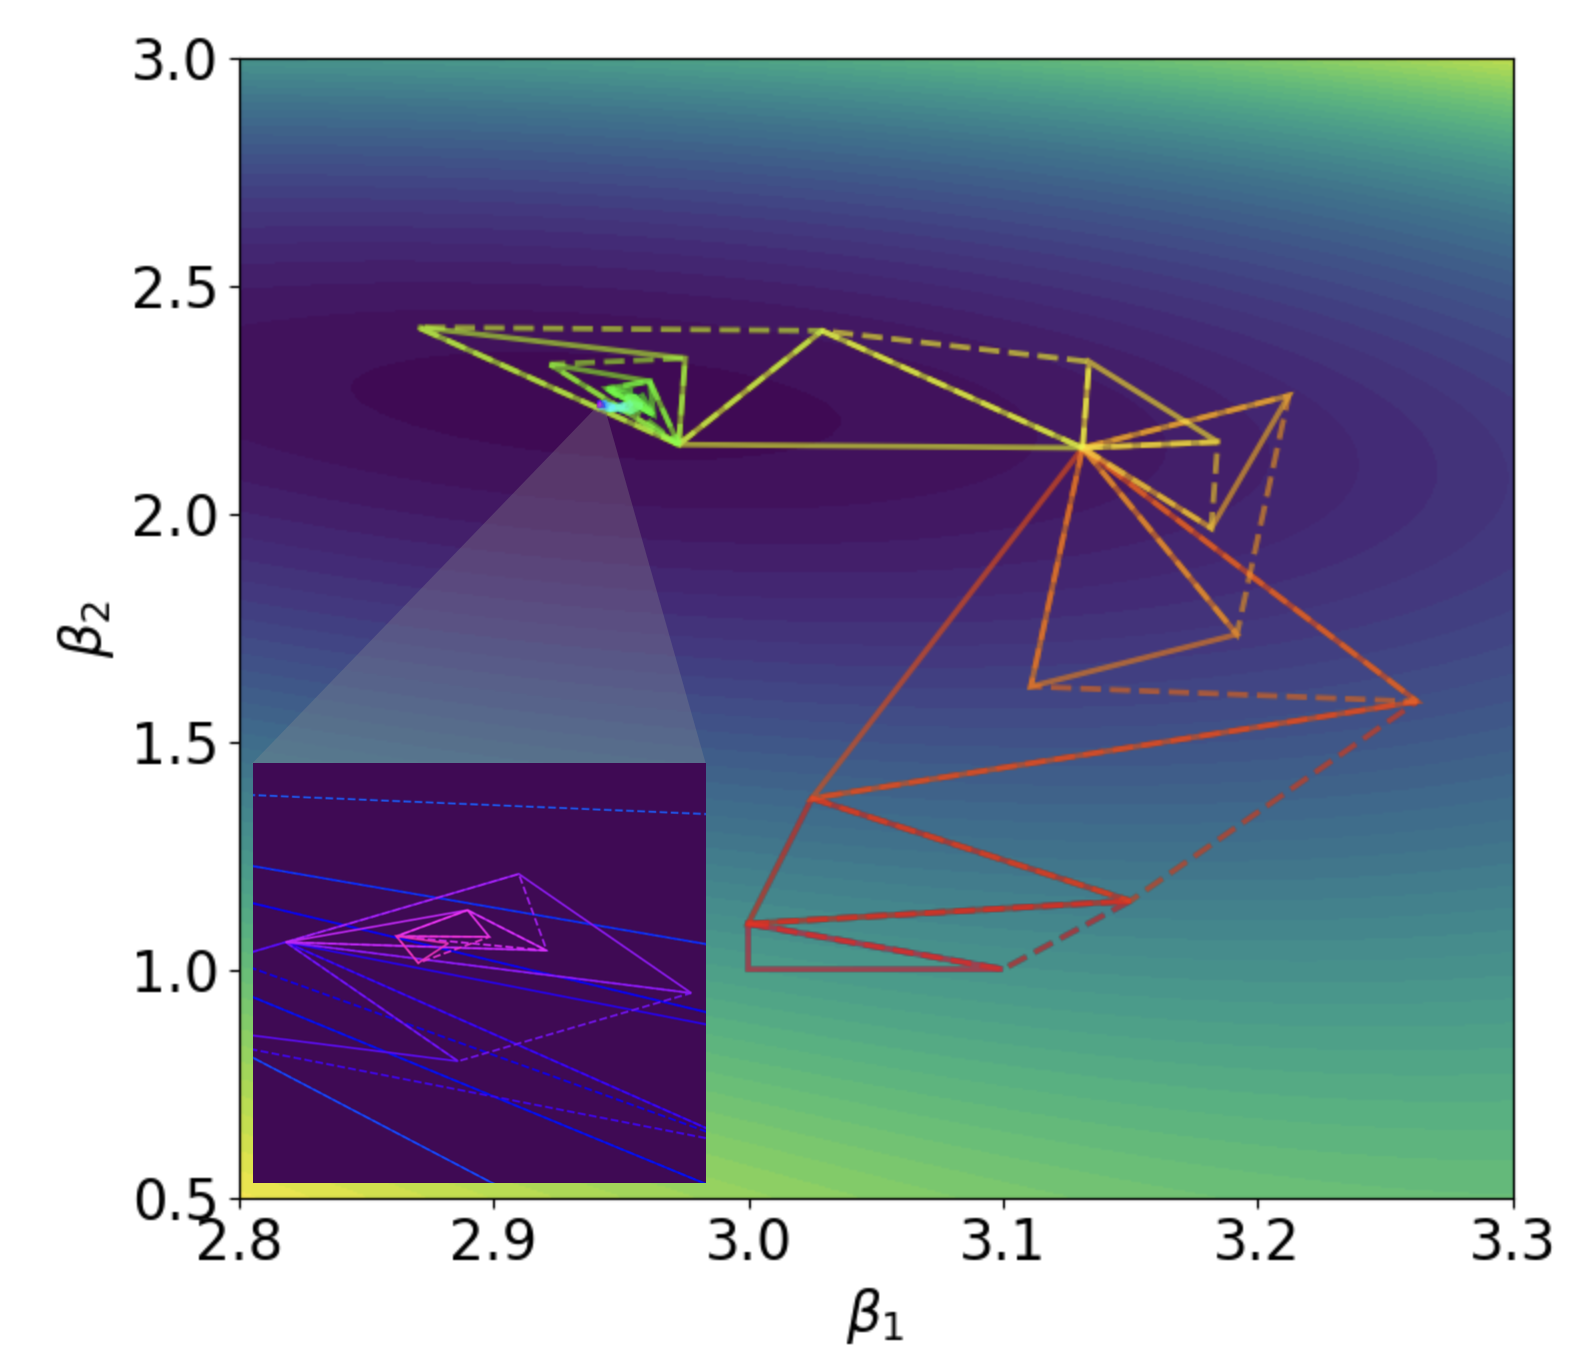
\includegraphics[width=0.6\linewidth]{images/nelder_mead_illustration.png} \caption[Visualising the Nelder-Mead optimisation algorithm.]{Illustration of the Nelder-Mead algorithm for a cost function parameterised by two parameters $\beta_1$ and $\beta_2$. The simplex for a 2-dimensional landscape is a triangle, which then follows the rough algorithm described in the text. The iterations of the algorithm are indicated by constantly switching from solid to dashed edges of the simplex at each step as well as changing in colour. The inset shows a magnification of the final steps of the algorithm.}\label{fig:nelder_mead}
\end{figure}

The way this direct search approach is adapted in Nelder-Mead is by constructing simplices, which are geometric objects that generalise triangles in lower and higher dimensions. For a cost function dependent on $n$ parameters, Nelder-Mead constructs an $n$-dimensional simplex. For $n=0$ this is a point, for $n=1,2,3$ a line segment, triangle and tetrahedron respectively and then higher-dimensional versions as $n$ increases. Thus a simplex has $n+1$ vertices for $n$ parameters. 

The vertices of this simplex then traverse the cost function landscape according to the Nelder-Mead algorithm in order to converge to some minimum value.  In most of the search steps, the primary change is to shift the highest point of the simplex (i.e., where the cost function value is largest) through the opposite face of the simplex, moving to a point with a lower cost function value. These steps are known as \emph{reflections} and they are designed to preserve the volume of the simplex, ensuring it remains non-degenerate. Whenever possible, the method will expand the simplex along a particular direction, which allows it to take bigger steps in search of a minimum. When the simplex encounters a region that can be thought of as a `valley floor' in the cost function landscape, it reduces its dimensions orthogonal to the valley, so that it can slide down. In situations where the simplex has to navigate through a narrow passage, it shrinks itself in all directions, wrapping itself around its best (lowest) point, enabling it to continue its search for the minimum. This process is illustrated for a simple example in Fig.~\ref{fig:nelder_mead}.

This description of the Nelder-Mead method is quite rough and it only covers the basic idea that was first developed in the original 1965 paper. Many variations and improvements have been developed in the years since and the actual implementations. In general, the Nelder-Mead approach is simple to understand and implement, as well as being quite efficient and flexible. However, it often suffers from convergence issues, being both likely to return a sub-optimal local minimum and to get stuck without converging far longer than necessary, undoing any efficiency it otherwise promised. Furthermore, the simplex method doesn't scale well in higher dimensions, making it less effective when the number of parameters is large.

\subsubsection{Powell's method}\label{sec:3.1.3.2_Powell}

Another approach from the gradient-free, local optimiser crowd is Powell's method, first developed by Michael J. D. Powell in 1964 \cite{powell_efficient_1964}. The algorithm is known as a \emph{conjugate-direction} approach, not to be confused with the more common conjugate-gradient approach, although the two are related as the latter can be viewed as a specialisation of the former. 

The basis of Powell's method relies on the idea of conjugate vectors or conjugate directions. Two vectors $\ubb$ and $\boldsymbol{v}$ are said to be conjugate with respect to some positive semi-definite matrix $A$ if $\ubb^T A \boldsymbol{v} = 0$. A set of conjugate directions, thus, is a set of vectors that are pairwise conjugate. Furthermore, one can make the observation \cite{brent_algorithms_2002} that the function
\begin{equation}
    f(\xbb) = \xbb^T A \xbb - 2\boldsymbol{b}^T \xbb + c
\end{equation}
for some positive semidefinite matrix $A$, $\boldsymbol{b} \in \R^n$ and $c \in \R$ has a minimum at the point $\sum_{i=1}^n \beta_i \ubb_i$ in the space spanned by the set of conjugate vectors $\{ u_j \}_{j = 1,...,n}$ with
\begin{equation}
    \beta_i = \frac{\ubb_i^T\boldsymbol{b}}{\ubb_i^T A \ubb_i}.
\end{equation}
This minimum can be calculated efficiently just through evaluating the function, without needing explicit access to $A$, $\boldsymbol{b}$ or $c$. This property allowed Powell to develop a simple but powerful gradient-free approach, which can be summarised as:
\begin{algorithm}
\caption{Powell's Method}
\begin{algorithmic}[1]
\Procedure{Powell}{}
\State Initialise the method with ansatz solution $\ubb_0 \in \R^m$ and $n \leq m$ conjugate search vectors $\{\xbb_1, ..., \xbb_n \}$. If none are provided, use columns of the $m$-dimensional identity matrix.
\For{$i = 1,...,n$}
\State Compute $\beta_i$ to minimise $f(\ubb_{i - 1} + \beta_i \xbb_i)$
\State Define $\ubb_i \gets \ubb_{i - 1} + \beta_i \xbb_i$
\EndFor
\For{$i = 1,...,n-1$}
\State $\xbb_{i} \gets \xbb_{i+1}$
\EndFor
\State $\xbb_n \gets (\ubb_n - \ubb_0)$
\State Compute $\beta$ to minimize $(f(\ubb_0  + \beta \xbb_n))$
\State $\ubb_0 \gets \ubb_0 + \beta \xbb_n$
\EndProcedure
\end{algorithmic}
\end{algorithm}
In other words,the algorithm is initialised with a guess and a set of conjugate directions. It then proceeds to find a minimum along each of the given directions, estimates the best potential direction to proceed in 

Disadvantages:

\begin{itemize}
    \item Computationally expensive: Powell's method can be more computationally expensive than gradient-based methods, especially for high-dimensional problems, as it requires multiple function evaluations for each line search.
    \item Convergence: The convergence rate of Powell's method is generally slower than that of gradient-based methods, particularly for well-conditioned problems.
    \item Sensitivity to initial conditions: The performance of Powell's method can be highly sensitive to the choice of initial starting point and the initial set of conjugate directions.
\end{itemize}

\subsubsection{Dual-annealing}\label{sec:3.1.3.3_dual_annealing}

Dual Annealing is a stochastic global optimization algorithm, effectively an implementation of the generalized simulated annealing algorithm \cite{tsallis_generalized_1996} along with 

It is an implementation of the generalized simulated annealing algorithm, an extension of simulated annealing. In addition, it is paired with a local search algorithm that is automatically performed at the end of the simulated annealing procedure.


\begin{figure}[t]
\centering
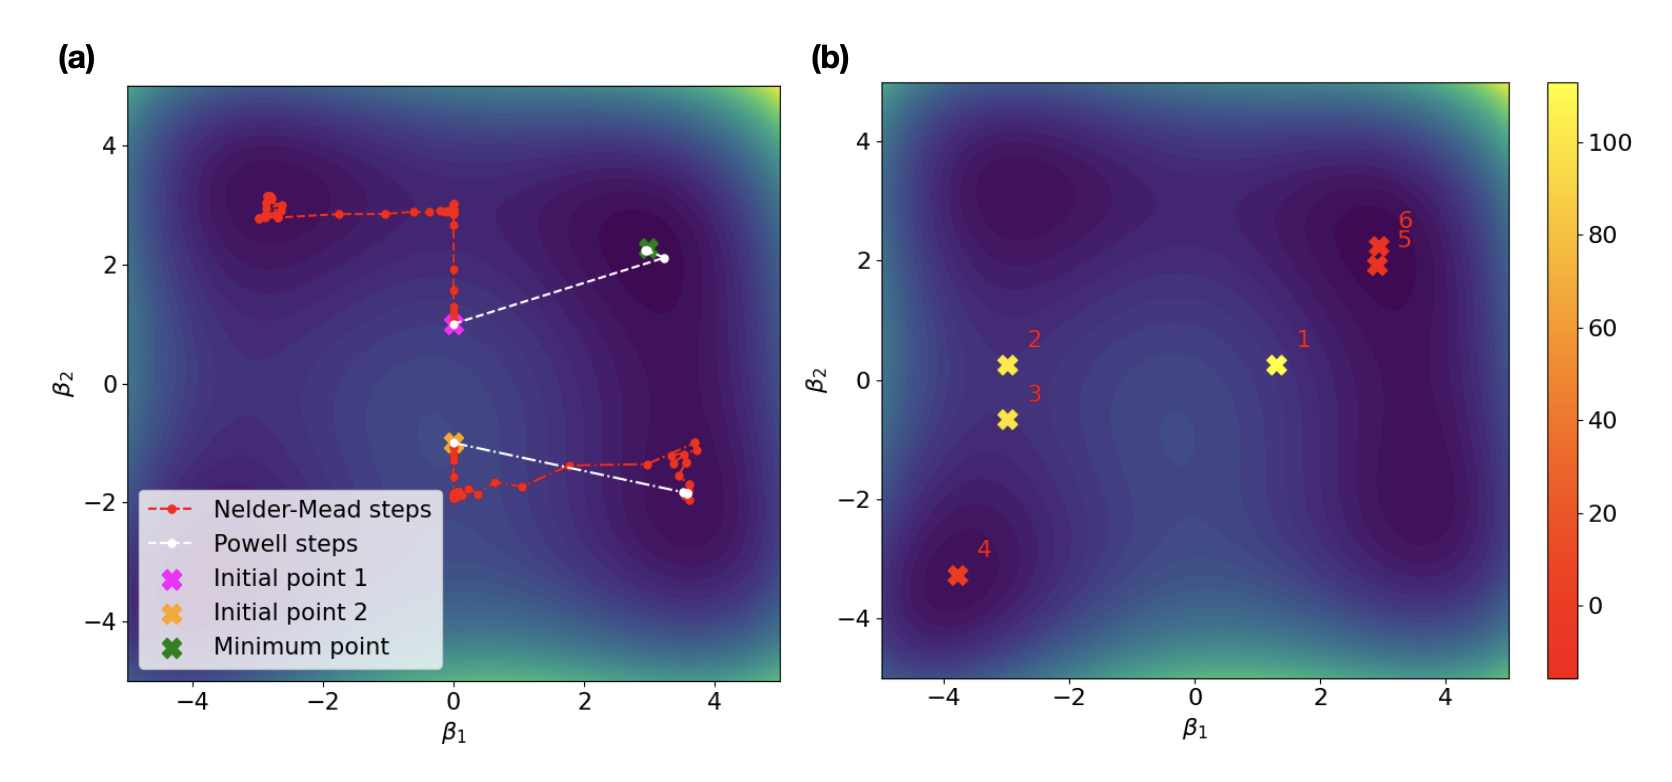
\includegraphics[width=\linewidth]{images/optimiser_plots.png} \caption[Visualising optimisers in action]{An illustration of the optmisation strategy of several numerical optimisation methods. (a) Local optimisers: steps of the Nelder-Mead method and Powell's method when instantiated in two different locations of the loss function landscape. The global mimimum is illustrated by a green cross. (b) The local minima (crosses) visited by the Dual-Annealing in the order indicated by the numbered labels. The color of the crosses reflects the value of the cost function evaluated at that point as indicated by the colorbar.}\label{fig:optimisers}
\end{figure}

Differences from other popular optimizers:

Global optimization: Unlike local optimization methods such as gradient descent, Newton's method, and conjugate gradient method, dual-annealing aims to find the global minimum of a function. This makes it more effective for non-convex optimization problems with multiple local minima.

Stochastic algorithm: Dual-annealing is a stochastic algorithm, meaning it incorporates random elements to explore the search space. This is in contrast to deterministic algorithms like gradient descent, which follow a fixed set of rules to update the search point.

Metaheuristic: Dual-annealing is a metaheuristic algorithm, inspired by the physical process of annealing in metallurgy. It combines simulated annealing and quantum annealing, both of which are also metaheuristics.

Advantages:

\begin{itemize}
    \item Global optimization: Dual-annealing is designed to find the global minimum of a function, making it suitable for optimization problems with multiple local minima.
    \item Robustness: Due to its stochastic nature, dual-annealing is less likely to get stuck in local minima compared to deterministic local optimization algorithms like gradient descent.
    \item Exploration and exploitation balance: Dual-annealing effectively balances exploration (searching for new promising regions) and exploitation (refining the current best solution) by adjusting its temperature parameters during the optimization process.
\end{itemize}

Disadvantages:

\begin{itemize}
    \item Computationally expensive: Dual-annealing can be computationally expensive, particularly for high-dimensional problems, as it requires a large number of function evaluations to explore the search space effectively.
    \item Convergence: The convergence rate of dual-annealing can be slower than gradient-based methods for well-conditioned optimization problems.
    \item Tuning parameters: The performance of dual-annealing can be highly sensitive to the choice of tuning parameters, such as the initial temperature and cooling schedule. It may require trial and error to find the best parameter settings for a particular problem.
\end{itemize}

In summary, dual-annealing is a global optimization algorithm that is well-suited for non-convex optimization problems with multiple local minima. It offers robustness and an effective balance between exploration and exploitation. However, it can be computationally expensive, have a slower convergence rate, and be sensitive to tuning parameters compared to other popular optimization techniques.

\section{Quantum optimal control}\label{sec:3.2_Quantum_optimal_control}

\reminder{Quantum optimal control theory (QOCT) refers to a set of methods to devise and implement shapes of external electromagnetic fields that manipulate quantum dynamical processes at the atomic or molecular scale in the best way possible}

In the quantum setting, the set of state functions $X$ often takes the form of a set of quantum states, be they complex vectors, density matrices or operators. The set of control functions $U$ is represented by a set of functions of parameterised Hamiltonians. It is common to decompose a control Hamiltonian into two components: the time-dependent `drive' part and the time-independent `drift' part. The time-dependent part can then be further decomposed into a set of $N_k$ operators $\{\mathcal{O}_{\rm opt}^{(k)}\}_{k=1,...,N_k}$, such that the full control Hamiltonian reads:
\begin{equation}
    H(\ubb(t)) = H_0 + \sum_{k = 1}^{N_k} u_k(t) \mathcal{O}_{\rm opt}^{(k)},
\end{equation}
where $H_0$ is the drift Hamiltonian with no external controls and the control functions $u_k(t) \in \ubb(t)$ drive the corresponding operators $\mathcal{O}_{\rm opt}^{(k)}$.

\begin{figure}[t]
\centering
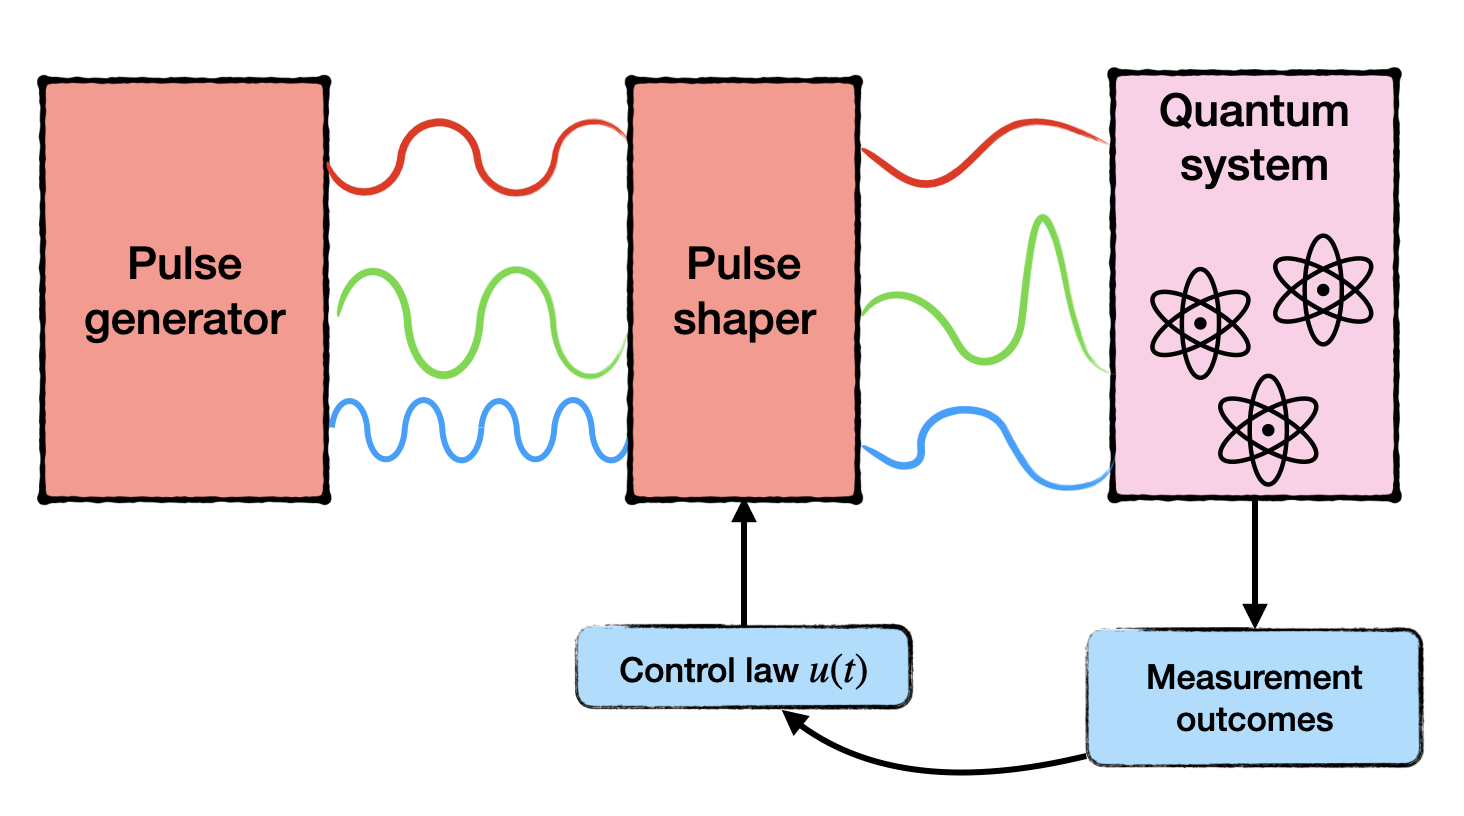
\includegraphics[width=0.8\linewidth]{images/optimal_control_placeholder.png} \caption[Schematic diagram of quantum optimal control]{An illustration of a general quantum optimal control problem set up. }\label{fig:quantum_optimal_control}
\end{figure}

Given this, we can describe a general quantum optimal control problem in analogy to Eq.~\eqref{eq:control_ODE} as one where the aim is to solve the Schr\"{o}dinger equation:
\begin{equation}
    i \hbar \partial_t \ket{\psi(t)} = H(\ubb(t))\ket{\psi(t)}
\end{equation}
with the constraint of starting in a state from a set of initial states $\ket{\psi_0} \in \boldsymbol \Psi_0$ and while minimising some cost function that targets a set of final states $\ket{\psi_T} \in \boldsymbol \Psi_T$.

The choice of cost function in the quantum setting is generally informed by the desired properties of the target state(s) combined with considerations for what information can be extracted from the system and other constraints. For example, when the aim of the optimisation is to prepare a single, well-defined quantum state $\ket{\psi_T}$ with high accuracy, then the most informative cost function is:
\begin{equation}\label{eq:costfunc_fidelity}
    C_F(\tau, \ubb) = 1 - F(\tau, \ubb) = 1 - \abs{\braket{\psi(\tau, \ubb)}{\psi_T}}^2,
\end{equation}
where $F(\tau, \ubb)$ is the fidelity of the final state $\ket{\psi(\tau, \ubb)}$ with respect to the desired target $\ket{\psi_T}$. Here $\ket{\psi(\tau, \ubb)}$ is generated by driving an initial state $\ket{\psi_0} \in \boldsymbol \Psi_0$ for a time $\tau$ via the time-dependent Hamiltonian $H(\ubb(t))$. If, on the other hand, the target state need only be a ground state of some Hamiltonian $H_T$, then it might be far more convenient to use the final system energy:
\begin{equation}\label{eq:costfunc_energy}
    C_E(\tau, \ubb) = \mel{\psi(\tau, \ubb)}{H_T}{\psi(\tau, \ubb)}.
\end{equation}
Finally, should one be interested only in a specific property of the final state, like its entanglement, then the cost function might look something like:
\begin{equation}\label{eq:costfunc_entanglement}
    C_S(\tau, \ubb) = -S[\ket{\psi(\tau, \ubb)}],
\end{equation}
where $S[\cdot]$ is some appropriate measure of entanglement. \reminder{add citations for examples where each is used?} As well as being informed by the set of target states, the cost function may include further constraints, like the total power of the driving fields in the Hamiltonian. This is analogous to the cost function in Eq.~\eqref{eq:example_cost_func2}, which in the quantum case might look something like:
\begin{equation}\label{eq:costfunc_constraint}
    C(\tau, \ubb) = C_F(\tau, \ubb) + \sum_{k = 1}^{N_k} \int_0^{\tau} \abs{u_k(t)}^2 dt,
\end{equation}
which can be read as an optimisation for final state fidelity with the added constraint that the fluences of the driving fields are minimised. 

\begin{mycolorbox}[box:reachability]{Reachability of state in the quantum setting}
    
\end{mycolorbox}

\reminder{Links to STA?}

\section{Methods}

Blah blah blah when it comes to quantum systems...

\subsection{Chopped random-basis quantum optimization (CRAB)}\label{sec:3.3.1_CRAB}

The ``Chopped random-basis quantum optimization" or \acrref{CRAB} method is a quantum optimal control method first introduced in \cite{doria_optimal_2011, caneva_chopped_2011} which revolves around the construction of a truncated randomized basis of functions for the control fields of a quantum system. It was devised as a means to overcome some of the complications and restrictions present in its contemporary approaches, which tended to be neither 

The key idea is to expand the control pulse $u(t)$ in some truncated basis of dimension $N_k$: 
\begin{equation}
    u(t) = \sum_{i = 1}^{N_k} c_i u_i(t),
\end{equation}
where the optimisation is then performed only on the coefficients $c_i$. 

The method in short:
\begin{enumerate}
    \item Initialization: Start by choosing an initial guess for the control fields, typically set to a constant value or initialized randomly.
    \item Random basis generation: Generate a random basis for each control field by selecting a set of random orthogonal vectors. The paper recommends using a Fourier basis and randomizing it through a linear transformation.
    \item Chopping: Divide the time interval of the control fields into several shorter subintervals (or chops). In each subinterval, the control fields are represented by a linear combination of the randomized basis functions.
    \item Optimization: Use a standard optimization algorithm to minimize the cost function. The cost function quantifies the deviation from the desired evolution of the quantum system. The optimization is performed with respect to the coefficients of the linear combinations, which represent the control fields in each subinterval.
    \item Iterative process: Iterate steps 2-4 until a satisfactory level of optimization is achieved.
\end{enumerate}

Advantages:

\begin{itemize}
    \item Enhanced exploration: The randomization of the control field basis allows for a more comprehensive exploration of the control landscape, which can lead to the discovery of better solutions.
    \item Improved convergence: The piecewise constant control fields enable the method to exploit local minima effectively, leading to faster convergence compared to other methods.
    \item Flexibility: The CRAB method can be applied to a wide range of quantum control problems, including those with constraints on the control fields or system parameters.
\end{itemize}

Disadvantages:

\begin{itemize}
    \item Additional complexity: The introduction of randomization and chopping adds complexity to the optimization process compared to traditional methods.
    \item Dependency on the optimizer: The efficiency and success of CRAB heavily depend on the choice of the optimization algorithm used in step 4.
    \item Convergence criteria: Determining an appropriate convergence criterion for terminating the iterative process can be challenging, as it may vary depending on the problem at hand.
\end{itemize}

Add in citations \cite{caneva_chopped_2011, muller_one_2022}

\subsection{Gradient Ascent Pulse Engineering (GRAPE)}\label{sec:3.3.2_GRAPE}

The ``Gradient Ascent Pulse Engineering" (GRAPE) algorithm is a widely used method for optimizing quantum control pulses in quantum computing and quantum information processing. The main goal of GRAPE is to determine control pulses that steer the quantum system from an initial state to a desired target state while minimizing a cost function. The algorithm iteratively refines the control pulses using gradient ascent optimization.

\reminder{can add some pseudocode across pages here}


\begin{enumerate}
    \item Initialization: Begin with an initial guess for the control pulses, which can be set to a constant value or initialized randomly.
    \item Propagation: Simulate the time evolution of the quantum system under the given control pulses to calculate the final state of the system.
    \item Cost function evaluation: Compute the cost function, which quantifies the deviation between the target state and the final state obtained in step 2. Common choices for the cost function are the fidelity or the infidelity between the two states.
    \item Gradient calculation: Compute the gradient of the cost function with respect to the control pulses. This is done by numerically evaluating the partial derivatives of the cost function with respect to each control pulse.
    \item Pulse update: Update the control pulses by following the gradient direction. This is typically done using a step size parameter that controls the magnitude of the pulse updates.
    \item Iterative process: Repeat steps 2-5 until the cost function reaches a satisfactory minimum value or a maximum number of iterations is reached.
\end{enumerate}

Advantages:

\begin{itemize}
    \item Robustness: GRAPE is known to be robust against local minima and typically converges to a global minimum for many quantum control problems.
    \item Efficiency: The algorithm is computationally efficient, as it only requires the calculation of the gradient of the cost function with respect to the control pulses.
    \item Wide applicability: GRAPE can be applied to a broad range of quantum control problems, including those involving constraints on the control pulses or system parameters.
\end{itemize}

Disadvantages:

\begin{itemize}
    \item Gradient calculation: The numerical calculation of the gradient can be challenging, particularly for systems with a large number of control pulses or complex dynamics.
    \item Convergence speed: The convergence rate of the GRAPE algorithm can be slow, especially if the initial guess for the control pulses is far from optimal.
    \item Dependency on the step size: The choice of the step size parameter can significantly affect the performance of the algorithm, with inadequate choices leading to slow convergence or oscillatory behavior.
\end{itemize}

Add in citations \cite{khaneja_optimal_2005}